\documentclass[aspectratio=169]{beamer}
	\usepackage[utf8]{inputenc}		% required for umlauts
	\usepackage[english]{babel}		% language
	%\usepackage[sfdefault]{roboto}	% enable sans serif font roboto
	%\usepackage{libertine}			% enable this on Windows to allow for microtype
	\usepackage[T1]{fontenc}		% required for output of umlauts in PDF

	\usepackage{mathtools}		% required for formulas

	\usepackage{caption}		% Customize caption aesthetics
	\usepackage{tcolorbox}		% fancy colored boxes
	\usepackage{xcolor}			% Highlighting
	\usepackage{soul}

	\usepackage{graphicx}		% required to insert images
	\usepackage{subcaption}		% enable sub-figure
	\usepackage[space]{grffile} % insert images baring a filename which contains spaces
	\usepackage{float}			% allow to forcefully set the location of an object

	\usepackage[tracking=true]{microtype} % required to change character spacing

	\usepackage[style=alphabetic,backend=biber]{biblatex}
	\usepackage{csquotes}		% ensure proper quotation of texts with babel and polyglossia with biblatex
	\usepackage{hyperref}		% insert clickable references

	\usepackage{datetime}		% flexible date specification
	\newcommand{\leadingzero}[1]{\ifnum#1<10 0\the#1\else\the#1\fi}
	\newcommand{\todayddmmyyyy}{\leadingzero{\day}.\leadingzero{\month}.\the\year}
	\newcommand{\mathcolorbox}[2]{\colorbox{#1}{$\displaystyle #2$}}

	\usepackage{geometry}
	\usepackage{scrextend}		% allow arbitrary indentation

	\usepackage{color}

	\makeatletter
	\let\@@magyar@captionfix\relax
	\makeatother

	\addbibresource{../literature.bib}

	\setbeamercolor{title}{fg=orange}
	\setbeamertemplate{title}{
		\color{orange}
		\textbf{\inserttitle}
	}
	\setbeamercolor{tableofcontents}{fg=orange}
	\setbeamercolor{section in toc}{fg=black}
	\setbeamercolor{subsection in toc}{fg=black}
	\setbeamertemplate{frametitle}{
		%\vspace{0.5em}
		\color{orange}
		\begin{center}
			\textbf{\insertframetitle} \\
			{\small \insertframesubtitle}
		\end{center}
	}
	\setbeamertemplate{footline}[text line]{
		\parbox{\linewidth}{
			\color{gray}
			\vspace*{-1em}
			NII 2018
			\hfill
			Gordian (\href{mailto:gordian.edenhofer@gmail.com}{gordian.edenhofer@gmail.com})
			\hfill
			\insertpagenumber
		}
	}
	\setbeamertemplate{navigation symbols}{}
	\setbeamertemplate{itemize item}{\color{black}$\bullet$}
	\setbeamertemplate{itemize subitem}{\color{black}$\circ$}
	\setbeamercolor{block title}{fg=black}
	\captionsetup{font=scriptsize,labelfont={bf,scriptsize}}

	\title{Update on `Meta-Learning~for~Recommender~Systems'}
	\subtitle{}
	\author[Edenhofer]{\href{mailto:gordian.edenhofer@gmail.com}{Gordian Edenhofer}}
	\institute[NII]{
		Working Group of Prof.~Dr.~Beel \\
		ADAPT Research Centre \\
		Trinity College Dublin
	}
	\date[Research Internship 2018]{\today}
	\subject{Natural Language Processing and Machine Translation}


\begin{document}
\section{Meta-Learning \\ ``learning to learn''}
\begin{frame}
	\frametitle{\insertsection}

	\begin{itemize}
		\item Ensemble learning
		\item Stacking
		\item Algorithm selection
	\end{itemize}
\end{frame}

\section{Meta-Learning}
\subsection{Motivation}
\begin{frame}
	\frametitle{\insertsection}
	\framesubtitle{\insertsubsection}

	\begin{figure}
		\centering
		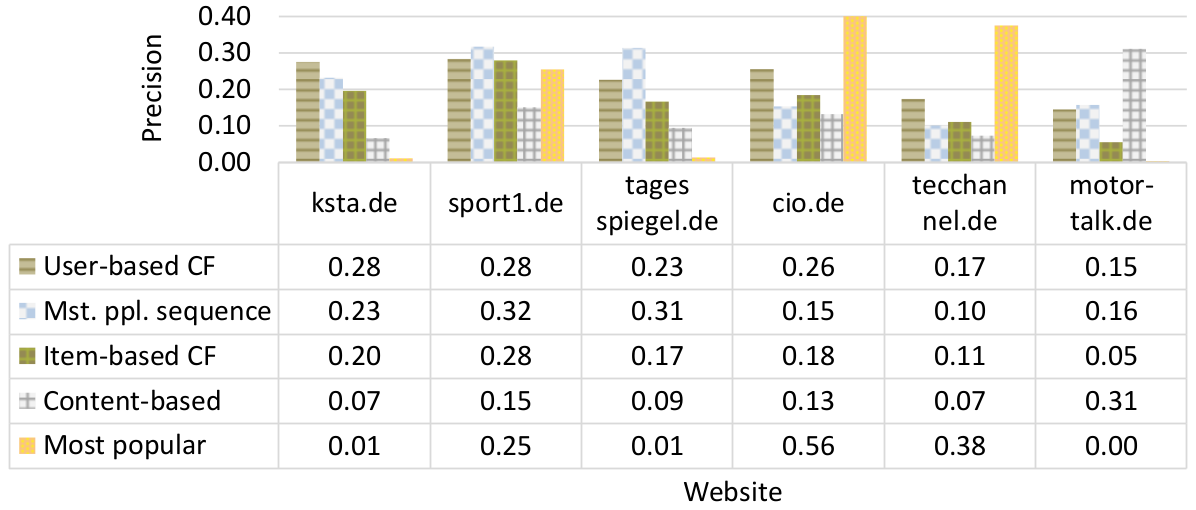
\includegraphics[width=\textwidth,height=0.6\textheight,keepaspectratio]{{{../res/Recommendation precision by new website - Andrew Collins}}}
		\caption{Recommendation precision by new website. Taken from~\cite{DBLP:journals/corr/abs-1805-12118}.}
	\end{figure}
\end{frame}

\subsection{Theoretical Best}
\begin{frame}
	\frametitle{\insertsection}
	\framesubtitle{\insertsubsection}

	\begin{figure}
		\centering
		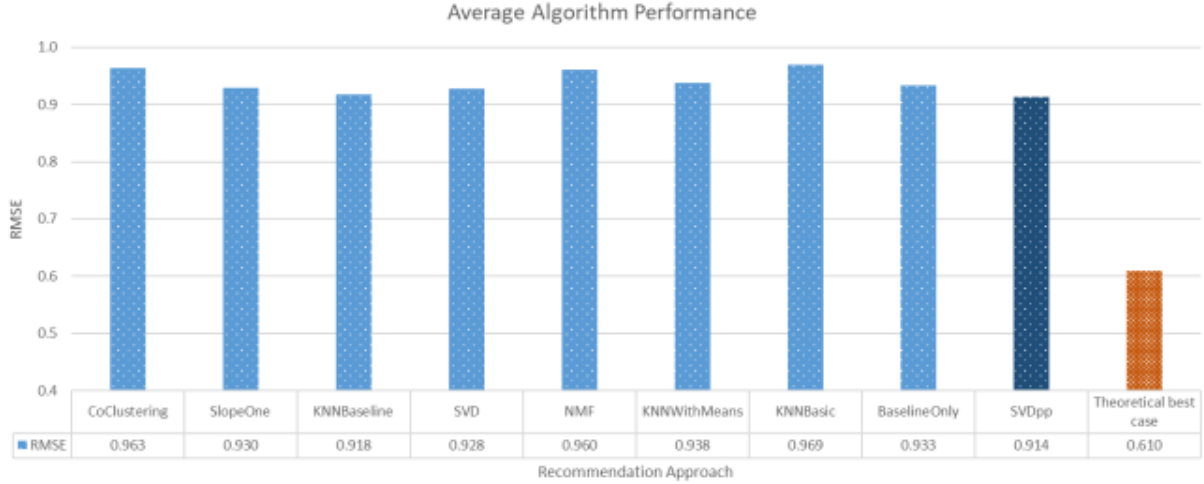
\includegraphics[width=\textwidth,height=0.6\textheight,keepaspectratio]{{{../res/RMSE by machine learning algorithm for MovieLense dataset with theoretical best meta-learner - Andrew Collins}}}
		\caption{RMSE by machine learning algorithm for MovieLense dataset with theoretical best meta-learner. Taken from~\cite{DBLP:journals/corr/abs-1805-12118}.}
	\end{figure}
\end{frame}

\begin{frame}
	\frametitle{\insertsection}

	\begin{itemize}
		\item Explored in related works as presented here
		\begin{itemize}
			\item MovieLense
			\item Yelp
			\item German news websites
		\end{itemize}
		\item Potential better candidates (more user-, item- and context information)
		\begin{itemize}
			\item DonorsChoose
			\item Stack Overflow
			\item LinkedIn user data (crawled by ADAPT group)
		\end{itemize}
	\end{itemize}
\end{frame}

\section*{Bibliography}
\begin{frame}
	\frametitle{\insertsection}

	\printbibliography
\end{frame}

\end{document}
